%! TeX program = lualatex

\documentclass[11pt]{extarticle}

% Set 1-inch margins
\usepackage[margin=1in]{geometry}

% Set Times New Roman for text and Cambria Math for math fonts
\usepackage{fontspec}
\setmainfont{Times New Roman}

% Use Symbol font for non-alphabetic characters
\usepackage{textcomp}

% Set line spacing to single (no less than single-spacing)
\usepackage{setspace}
\setstretch{1.0}

% Package for handling citations
\usepackage[backend=biber,style=numeric,sorting=none]{biblatex}
\addbibresource{references.bib}

% For inserting images and subcaptions
\usepackage{graphicx,subcaption} 
\usepackage{wrapfig}
\usepackage{svg}

% Begin document
\begin{document}

\textbf{Graduate Research Plan Statement}

\textbf{Introduction and Background:} The goal of this proposal is to demonstrate how category theoretic treatments of knowledge discovery processes can improve the fundamental understanding of relationships between such processes, reduce time needed to find relationships, and how processes can be resused for novel applications.
Central to these goals is the idea of compositionality: the characteristic that describes and quantifies how complex things can be assembled out of simple parts [1].
This is a concept common across mathematics but is seen frequently in the fundamentals of category theory.
Simply put, category theory studies the relationships that exist between things which gives a vantage point to think not on the details of a particular problem but more broadly about how things in a problem space may fit together (i.e. be composed).
Category theory is primed to take advantage of ideas shared across domains such as knowledge discovery, the process of scrutinizing available data to generate novel insight about a particular field or topic. % TEJA: Does this seem natural?

\begin{wrapfigure}{r}{0.3\textwidth}
\centering
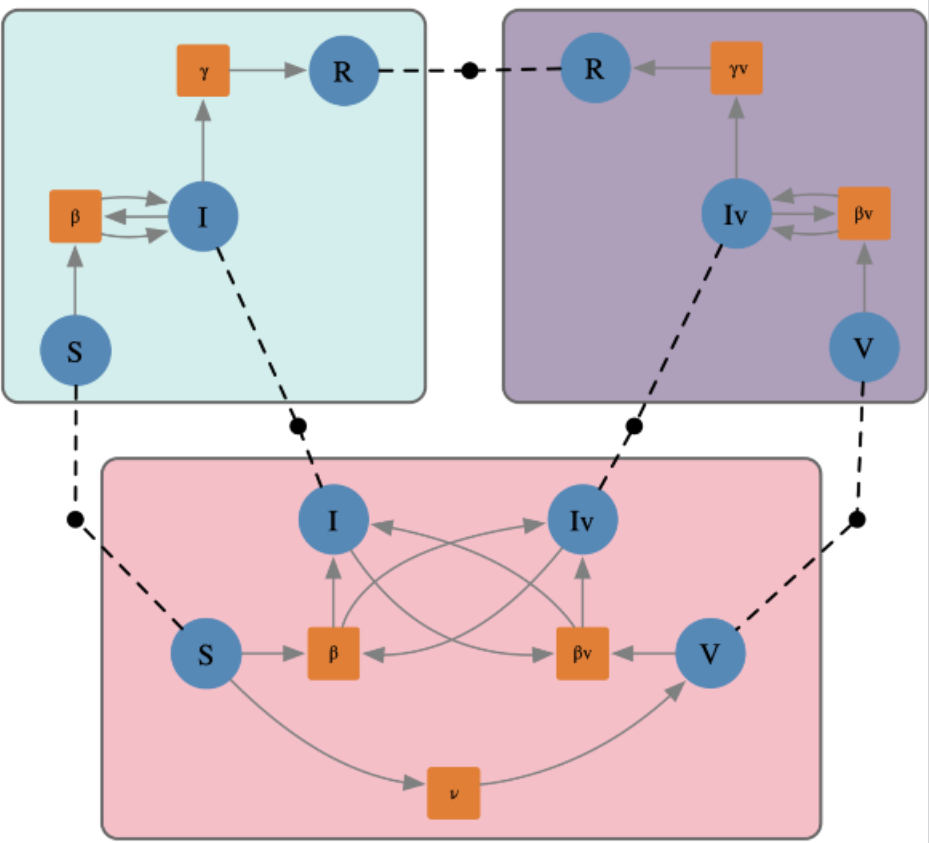
\includegraphics[width=0.3\textwidth]{sub_models}
\vspace{-15pt}
\caption{
  3 discovery processes (the three different petri nets in boxes) with relationships defined by arrows and lines inside of and between processes. % TEJA: How does caption read?
}
\vspace{10pt}
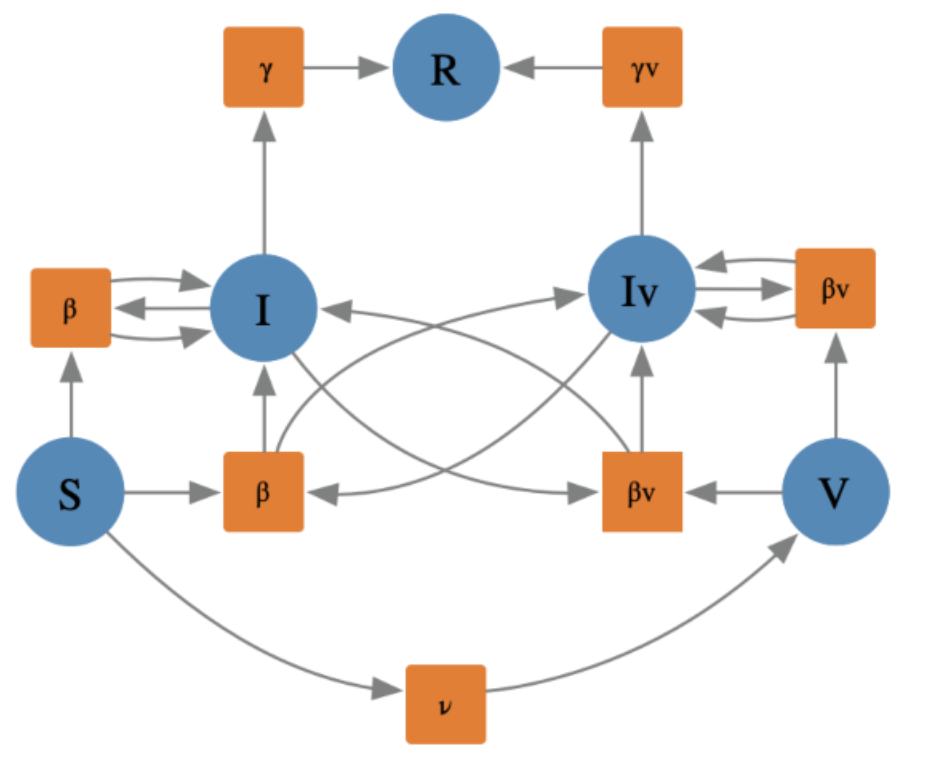
\includegraphics[width=0.25\textwidth]{composed_model}
\vspace{-10pt}
\caption{
  Composition of the 3 discovery processes into one novel discovery process. % TEJA: How does caption read?
}
\end{wrapfigure}

My experiences at Georgia Tech Research Institute and the US Centers for Disease Control motivated this proposal as I noticed knowledge discovery can be similar across disciplines.
However, due to domain specifics, adapting old proccesses to novel needs can be a labor intensive and time consuming process. 
To give an example, petri nets, which are well-studied in category theoretic terms, can be used to diagram dynamical systems as shown in Figure 1 [2].
Within each box in Figure 1, the petri nets represent the dynamical systems given by variations on a compartmental model.
In Figure 1, circles represent populations, squares represent variables that weaken the strength of the relationships given by arrows between populations, and dotted lines relate populations across the three processes.
Figure 2 then shows the result of how composing these models across dotted lines can reuse separate knowledge discovery processes while also simplifying them into one novel process subsuming former procceses.

\textbf{Research Plan:} At Harvard University, I will pursue a PhD to investigate the category theoretic understanding of knowledge discovery under Professor Nathaniel Osgood.
Additionally, I will continue my collaboration relationships with the Topos Institute and the University of Florida GATAS Lab who are pioneering applied category theory approaches and technologies.

\textbf{Objective 1: Map the Knowledge Discovery Process to Category Theoretic Language.} To investigate the general knowledge discovery process, I will pick three heterogeneous data sets that vary by how they are sampled over time and by what kind of data they contain. 
Then, I will construct general knowledge discovery proccesses to scrutinize these data sets.
This will be done through data science techniques such as clustering or prediction methods in order to simulate deriving novel insights about data.

Once several relationships that exist within and between data sets have been uncovered, I will then proceed to map these knowledge discovery processes on to various categorical structures.
First, I will use $\mathscr{C}$-sets, which describe a functor mapping a schema category $\mathscr{C}$ into the category $\mathbb{Set}$ (as objects) and the functions between them (as morphisms) [3].
Then, to assess how reasonable the identified relationships are, I will use a decorated copresheaf structure (known as acsets) to compute a presentation of the schema represented by the acset [4].
This objective will be completed when I have created an adequate $C$-set presentation that describes the relationships present within and between these datasets.

\textbf{Objective 2: Prototype Knowledge Discovery for a Specific Topic Using Category Theoretic Framing.} As the data sets are now framed in category theoretic terms, I will develop a knowledge discovery process adapted to an open topic relevant to these data sets.
Using tools from AlgebraicJulia, an open source research software stack based on category theoretic structures [5], I will determine what metrics and statistics are possible to compute on this framing by taking inspiration from previous work done by Dr. Libkind [2] and Prof. Osgood [6].
Objective 2 will be completed once I have determined what methods are most applicable to this framing and have formulated questions unique to this categorical framing.

\textbf{Objective 3: Optimizing the Composition of Knowledge Discovery Processes.} At this stage, I will do objectives 1 and 2 again to construct a different $C$-set presentation for another knowledge discovery process on top of the same datasets currently being used for investigation.
Once this other knowledge discovery process has been completed, I am now at the most crucial part of this effort: determining how to optimally compose knowledge discovery processes.
I will define the relationships that can exist throughout these processes (as in Figure 1) and then determine how to compose and simplify these processes into a novel discovery process (as in Figure 2).
Objective 3 will be completed when I have, in a similar manner to objective 2, decided what metrics I can compute upon this composed structure and determine what novel insight this new process uncovers within the topic of investigation.

\textbf{Intellectual Merit:} By using category theory to frame knowledge discovery involving heterogeneous datasets, data harmonization can become a simpler process than investigation of data sets via traditional data science practices.
As can be seen in Figures 1 and 2, relationships are much more clear across discovery processes and is easier to track the complexities of large processes or the compositions thereof with this framing.
In this way, the time cost of understanding and repurposing old processes could be greatly reduced and can lead to quicker insights into new problems rather than in an ad hoc manner of testing various data science methods against a data set or collection of data sets.

\textbf{Broader Impacts:} Category theory has a long history of application with database architecture [7] and is also finding applications within engineering system design [8] and machine learning [9].
By pursuing this work, I will be at the forefront of these emerging applications and can expand how complex knowledge discovery systems can be understood and analyzed across various disciplines.
Furthermore, this work could improve the construction of discovery processes from inception by allowing easier reasoning through how developing processes could be composed in the future or with other processes while in development leading to these knowledge discovery processes potentially being reduced from weeks to a matter of days [10].
Finally, as I will be exploring the limits of the available category theoretic machinery through this work, I will be in the ideal position to investigate new frontiers in applying category theory whether through informing the foundational mathematics of category theory or in the development of new open source research software that can be reused and developed further within the category theory community.

\textbf{References:} [1] \textit{Compositionality}, 2024. [2] \textit{An Algebraic Framework for Structured Epidemic Modelling.}, Libkind, et. al., 2022. [3] \textit{Categorical Software Engineering for Dynamic Simulation Modeling in Systems Science}, 2024. [4] \textit{Categorical Data Structures for Technical Computing}, Lynch, et. al., 2021. [5] \textit{AlgebraicJulia: a compositional approach to technical computing}, Patterson, 2022. [6] \textit{ModelCollab}, Baez, et. al., 2024. [7] \textit{Algebraic Databases}, Shultz, et. al., 2016. [8] \textit{ACT4ED}, MIT 1.S980, 2024. [9] \textit{Category theory in machine learning}, Gavranović, 2021. [10] \textit{Measuring the impact of knowledge loss: a longitudinal study}, Massingham

\end{document}
